
%%%%%%%%%%%%%%%%%%%%%%% file typeinst.tex %%%%%%%%%%%%%%%%%%%%%%%%%
%
% This is the LaTeX source for the instructions to authors using
% the LaTeX document class 'llncs.cls' for contributions to
% the Lecture Notes in Computer Sciences series.
% http://www.springer.com/lncs       Springer Heidelberg 2006/05/04
%
% It may be used as a template for your own input - copy it
% to a new file with a new name and use it as the basis
% for your article.
%
% NB: the document class 'llncs' has its own and detailed documentation, see
% ftp://ftp.springer.de/data/pubftp/pub/tex/latex/llncs/latex2e/llncsdoc.pdf
%
%%%%%%%%%%%%%%%%%%%%%%%%%%%%%%%%%%%%%%%%%%%%%%%%%%%%%%%%%%%%%%%%%%%


%\documentclass[runningheads,a4paper]{llncs}
\documentclass[a4paper]{./plantillas/llncs}

\usepackage{amssymb}
\setcounter{tocdepth}{3}
\usepackage{graphicx}

\usepackage{url}
\urldef{\mailsa}\path|{jmanuel, gonzalo}@bacchuss.com.ar|    
\newcommand{\keywords}[1]{\par\addvspace\baselineskip
\noindent\keywordname\enspace\ignorespaces#1}

%JMANUEL
\usepackage[utf8]{inputenc}  %con el formato de applemac no andan los acentos directos.
\usepackage[spanish]{babel}

%JMANUEL NOTAS:
% Para poner txt en itálicas: \emph{palabra}



\begin{document}

\mainmatter  % start of an individual contribution

% first the title is needed
\title{VIDIX - Detección Visual de Intrusos en Redes de Datos}

% a short form should be given in case it is too long for the running head
%\titlerunning{Lecture Notes in Computer Science: Authors' Instructions}

% the name(s) of the author(s) follow(s) next
%
% NB: Chinese authors should write their first names(s) in front of
% their surnames. This ensures that the names appear correctly in
% the running heads and the author index.
%
\author{Juan Manuel Ramon Mosso, Gonzalo Buszmicz}
%
\authorrunning{Lecture Notes in Computer Science: Authors' Instructions}
% (feature abused for this document to repeat the title also on left hand pages)

% the affiliations are given next; don't give your e-mail address
% unless you accept that it will be published
\institute{Bacchuss, Investigación y Desarrollo,\\
Sarmiento 537 PB B., 2000 Rosario, Santa Fe, Argentina\\
\mailsa\\
\url{http://www.bacchuss.com.ar}}

%
% NB: a more complex sample for affiliations and the mapping to the
% corresponding authors can be found in the file "llncs.dem"
% (search for the string "\mainmatter" where a contribution starts).
% "llncs.dem" accompanies the document class "llncs.cls".
%

\toctitle{Lecture Notes in Computer Science}
\tocauthor{Authors' Instructions}
\maketitle


\begin{abstract}
La dependencia en las TIC como uno de los pilares fundamentales para el desarrollo social, económico y militar... \newline 

{\bfseries Palabras clave:} análisis visual, fusión de datos, seguridad, redes de datos 

\end{abstract}



\section{Introducción}

La dependencia en tecnologías de información y comunicaciones como uno de los pilares fundamentales para el desarrollo social, económico y militar de las naciones y corporaciones,  junto a la tendencia acentuada en el número de redes y servicios conectados a Internet generan un incremento considerable en los niveles de riesgo de seguridad asociados a los datos y servicios de TI...

\section{El Problema}

La  problemática abordada en el presente trabajo consiste en la optimización del proceso de análisis de grandes volúmenes de información vinculada con la protección de infraestructuras de TIC por medio de la creación de un sistema de información que favorezca el CS. La primera cuestión a analizar consiste en la comprensión del ciclo de vida de producción de información relacionada con eventos de seguridad. A tal fin se presenta un modelo para gestión de incidentes conformado por cinco procesos \cite{b1}, cada uno de los cuales cumple una función altamente especializada en base a los objetivos de negocios de la organización:


\begin{enumerate}
\item {\bfseries Preparación:} establecimiento, implementación y sostenimiento de un esquema de trabajo y de mejora continua sobre el grupo de respuesta a incidentes de seguridad.
\item {\bfseries Protección:} implementación de planes de acción y de mejora en cuanto a protección de la infraestructura con el fin de mitigar los riesgos de seguridad existentes...
\end{enumerate}


En la Figura 1 puede verse un esquema del modelo mencionado. \newline

\begin{figure}
\centering
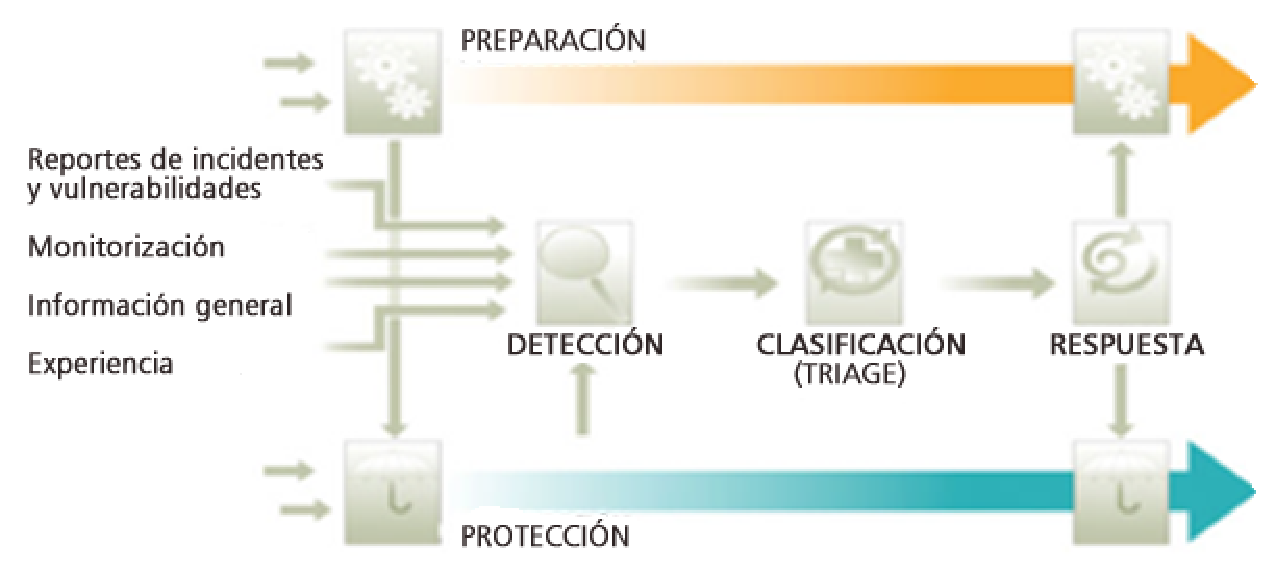
\includegraphics[scale=0.4]{./img/1-gis}
\caption{Modelo de precesos para Gestión de Incidentes de Seguridad (GISeg)}
\end{figure}


Para dar una idea de la complejidad del problema de procesamiento de alertas...



\section{Solución y Prototipo}

Dar solución a las problemáticas planteadas enla sección anterior requiere previamente de un estudio del rol de los diferentes actores intervinientes en el problema de seguridad en infraestructuras de TIC por lo que deben ser analizados tanto los componentes objetivo de ataques y sus aplicaciones y servicios vinculados, como los atacantes, sus organizaciones, motivaciones, ubicación geográfica, herramientas utilizadas, y si resulta posible sus motivaciones y relaciones...

\subsection{Requerimientos del prototipo}

Para el desarrollo del prototipo se pensó en una serie de requerimientos, los cuales pueden ser agrupados en dos tipos: funcionales y visuales...

\subsection{Aproximación a la Solución}

La definición de CS mas relevante a los objetivos del presente trabajo puede sintetizarse de la siguiente manera: CS consiste en la percepción de los elementos en un dominio determinado, dentro de un volumen determinado de tiempo y espacio, la comprensión de su significado, y la proyección de su situación en el futuro cercano \cite{b2}...

Si bien existen mecanismos alternativos para la reducción de los volúmenes de información como por ejemplo los lenguajes de correlación como LUA \cite{b3}, y otros \cite{b4} \cite{b5} \cite{b6}, y la asistencia mediante sistemas inteligentes \cite{b7} \cite{b8} \cite{b9} \cite{b10}, en este trabajo se probará la potencialidad del AV... 





\begin{thebibliography}{4}

\bibitem{b1} Ramon Mosso, J.M.: Modelo de Gestión de Incidentes de Seguridad (2008). Bacchuss.

\bibitem{b2} Endsley, M.R.: Toward a theory of situation awareness in dynamic systems. Human Factors 37(1), 32–64. (1995)

\bibitem{b3} LUA programming Languaje. \url{http://www.lua.org/about.html}

\bibitem{b4} Abadyz C., Taylory J., Senguly C., Yurcikz W., Zhouy Y., Rowex K.: Log Correlation for Intrusion Detection: A Proof of Concept.

\bibitem{b5} Kruegel C., Valeur F., Vigna G.: Intrusion Detection and Correlation - Challenges and Solutions.
Series: Advances in Information Security, Vol. 14 (2005)

\bibitem{b6} Cuppens F., Miège A.: Alert Correlation in a Cooperative Intrusion Detection Framework
ONERA Centre de Toulouse, 2, av. Edouard Belin, 31005, Toulouse CEDEX, France

\end{thebibliography}


\end{document}
